\documentclass[../main.text]{subfiles}
\begin{document}

%%find a citation that talks about categorical data in set theoretic terms

Categorical data can be likened to set measurment, where each category is a set
and researchers often want to know how many members each set has and what
intersections are common between sets. It is the latter that is analogous to a
conditional probability, the question of the likelihood of membership in one
set given membership in another. And sometimes there is also a quantative
component involved too. For example, in a study of how NEH funding has changed
over time, there are questions of the likelihoods of different disciplines
being funded (\{d_0,\dots,\d_i}\in \D), and if that is conditioned on institutione
  type \{i_0, \dots,\i_n}\in I}, and if either of those are then conditional on time \{t_0, \dots,t_n} \cite{wired} 
%% this can as easily be 311 data, but I don't have a citation for that
 The most common approach is usually to create a list of frequncies, sometimes of
 sets of one category, such as \D, or a crosstable wherein each cell is a an element
 in the product of two (or more sets), such as \D\cross \I creates a table
 wherein cell one is the frequency of elements that are in both $\d_0$ and
 $\i_0$ \cite{what is cross tabulation?}

 While a table is encouraged for a small number of variables
 \cite{munznertablesgood}), bar graphs and histograms are typically used to display
 differences between subsets such as \d_0,\dots, \d_n
 \cite{ioannidis_history_2003-1, friendly_brief_2006}. Variations on histograms
 include the hanging rootgram, ord plot, and other distribution oriented
 plots \cite{tukey_exploratory_1977, friendly_visualizing_2000}. While conditional  distributions can somewhat be visualized using Fourfold displays, Mosiac displays, and using logit models, these plots have somewhat limited dimensionality and are somewhat limited to 3 sets of categories
 \cite{friendly_visualizing_2000}. 
   
 
 \begin{figure}
   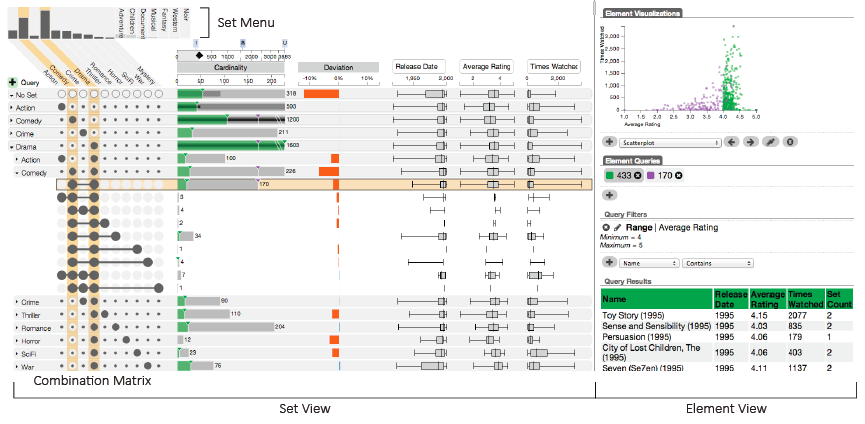
\includegraphics{upsetfig1}
   \caption{UpSet dashboard displaying the relationships amongst movie
     genres. On the left is the set visualiztion; the columns are the sets and
     the rows are the exclusive intersections or aggregates. On the right is
     the element view, and the scatter plot is a comparison of two sets with
     each dot equaling one element in the set.}
   \label{fig:upsetfig1}
 \end{figure}

The UpSet tool is designed to
display a much larger number of set intersections and the aggregate
information of quantative attributes and set membership. \cite{lex_upset:_2014}
As shown in figure~\ref{fig:upsetfig4}, the Upset tool provides linked set and element views. The set view provides the intersections and their
aggregates, the frequencies of each set and intersection, and the aggregate
statistics of the associated quantative variables, while the element view shows
selected elements and information about their set membership. The Upset tool
also faciliatates comparison of filtered sets via scatterplot, which acts as a
visualization of the attributes of the data conditioned on membership in the
filtered set.  

\begin{figure}
  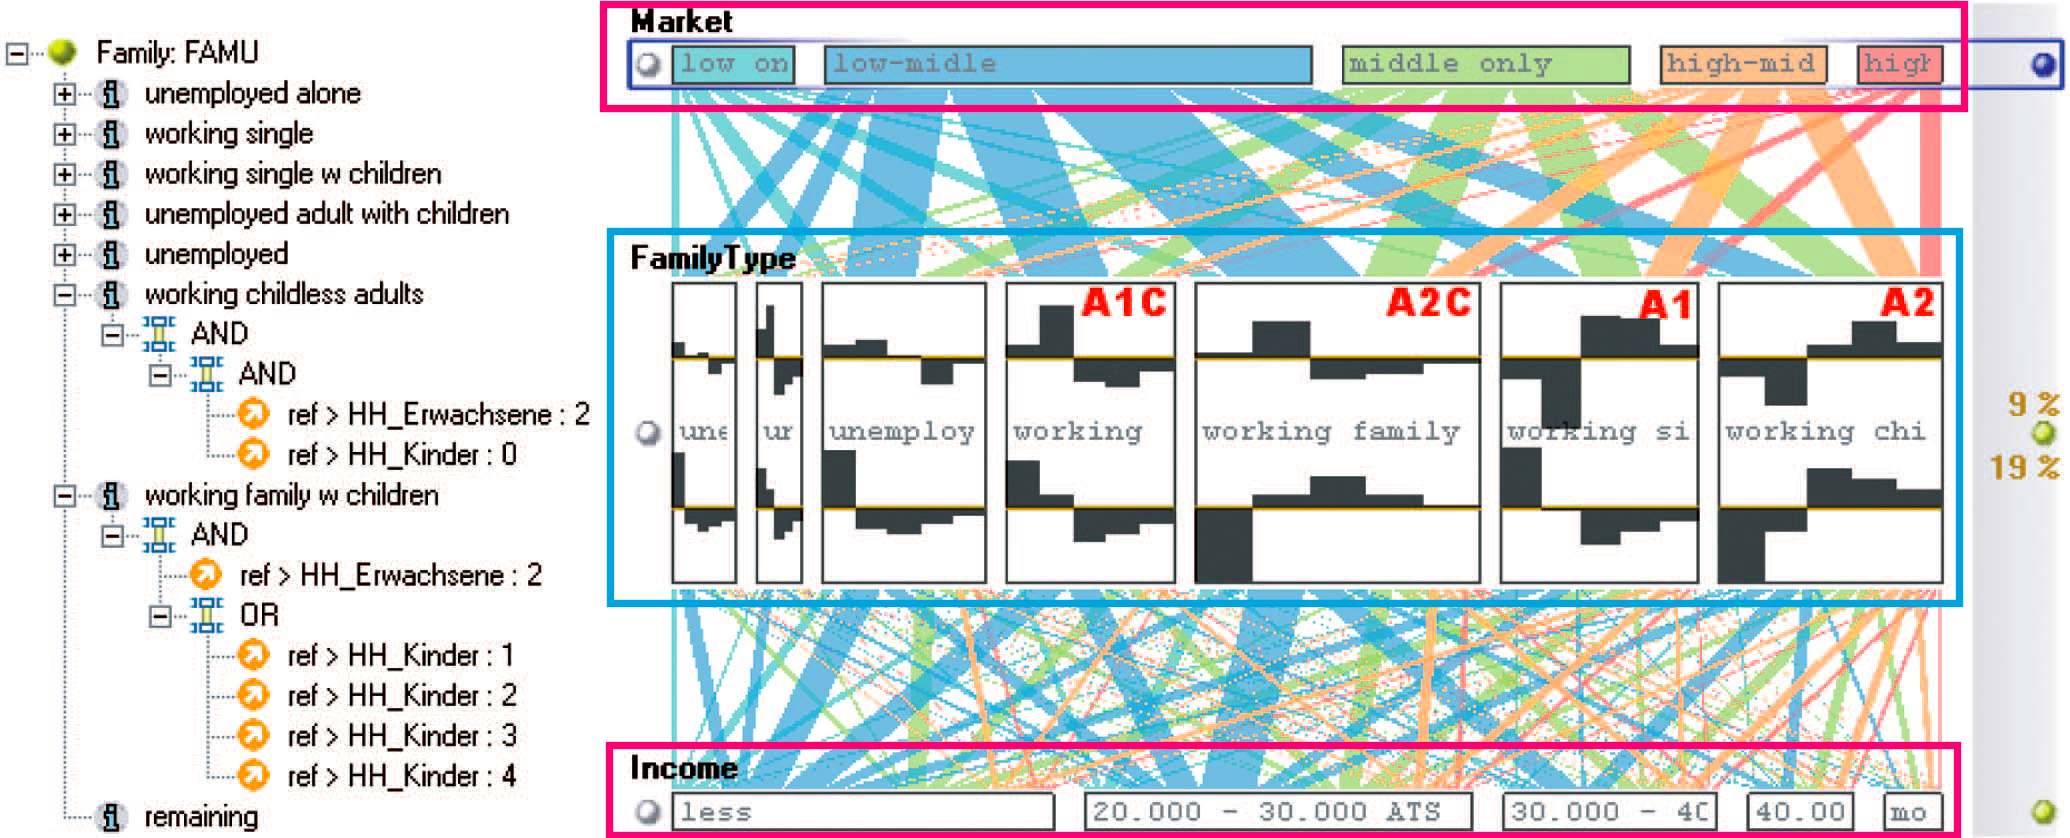
\includegraphics{parallelsets.png}
  \caption{On the left is the categorical view, where users can define
    categories based on other categorical information. For example, in this
    veiw working family with children is defined as a household with one or
    more children. On the right is a parallel coordinate graph wherin the
    dominiant category informs the colors, the size of the box is relative to
    ghe category size, and the historgrams show the freqiencies of those
    categories relative to the connecting catgories (market type and income
    respectively). }
  \label{fig:upsetfig1}
\end{figure}

Another important factor in visualizing categorical data is retaining the
inherent heirachy in many datasets with categorical measurements
\cite{shneiderman_visualizing_2000}. The Parallel Sets tool
showin in figure~\ref{fig:upsetfig} is expicilitly designed to show frequencies
of set membership in heirarichal ordered categorical sets, so the \{d_0, \dots, d_n} \in D
  \cite{kosara_parallel_2006}. Building on the fexible linked axis version of
  the parallel cooridnates plot \cite{flexible linked axis}, Parallel Sets
  treats each categorical set independantly but indicates conditional
  dependency through cross tabulations and by grouping the data, indicated via
  color, based on an active dimension that then becomes the pivot point for the
  cross tabulations. In Parallel Sets, quantative data is converted to
  categorical via binning.

\begin{figure}
    
\end{figure}
Often though it's important to retain the internel structure of the
quantative data, such as when it has internal structucture such as time and
space. Zhang et al propose a method that retains data and allows for
visualizing more than just pairwise relationships\cite{zhang_visual_2015}. Thei

\end{document}
